% !TEX TS-program = pdflatex
% !TEX encoding = UTF-8 Unicode

% This is a simple template for a LaTeX document using the "article" class.
% See "book", "report", "letter" for other types of document.

\documentclass[12pt]{article} % use larger type; default would be 10pt

\usepackage[utf8]{inputenc} % set input encoding (not needed with XeLaTeX)

%%% Examples of Article customizations
% These packages are optional, depending whether you want the features they provide.
% See the LaTeX Companion or other references for full information.

%%% PAGE DIMENSIONS
\usepackage{geometry} % to change the page dimensions
\geometry{a4paper} % or letterpaper (US) or a5paper or....
\geometry{margin=1in} % for example, change the margins to 2 inches all round
% \geometry{landscape} % set up the page for landscape
%   read geometry.pdf for detailed page layout information

\usepackage{graphicx} % support the \includegraphics command and options

% \usepackage[parfill]{parskip} % Activate to begin paragraphs with an empty line rather than an indent

%%% PACKAGES
\usepackage{booktabs} % for much better looking tables
\usepackage{array} % for better arrays (eg matrices) in maths
\usepackage{paralist} % very flexible & customisable lists (eg. enumerate/itemize, etc.)
\usepackage{verbatim} % adds environment for commenting out blocks of text & for better verbatim
\usepackage{subfig} % make it possible to include more than one captioned figure/table in a single float
% These packages are all incorporated in the memoir class to one degree or another...
\usepackage{float}

%%% HEADERS & FOOTERS
\usepackage{fancyhdr} % This should be set AFTER setting up the page geometry
\pagestyle{fancy} % options: empty , plain , fancy
\renewcommand{\headrulewidth}{0pt} % customise the layout...
\lhead{}\chead{}\rhead{}
\lfoot{}\cfoot{\thepage}\rfoot{}

%%% SECTION TITLE APPEARANCE
%\usepackage{sectsty}
%\allsectionsfont{\sffamily\mdseries\upshape} % (See the fntguide.pdf for font help)
% (This matches ConTeXt defaults)

%%% ToC (table of contents) APPEARANCE
\usepackage[nottoc,notlof,notlot]{tocbibind} % Put the bibliography in the ToC
\usepackage[titles,subfigure]{tocloft} % Alter the style of the Table of Contents
\renewcommand{\cftsecfont}{\rmfamily\mdseries\upshape}
\renewcommand{\cftsecpagefont}{\rmfamily\mdseries\upshape} % No bold!

%%% END Article customizations

\usepackage{xcolor}
\usepackage{graphicx}
\usepackage{siunitx}
\usepackage{url}
\usepackage{hyperref}
\graphicspath{ {./images/} }

%%% The "real" document content comes below...

\title{Controlling an Animatronic Chimpanzee Head}
\author{
	Jesse Patrick Sheehan \\
	\textit{Department of Electrical and} \\
	\textit{Computer Engineering} \\
	\textit{University of Canterbury}\\
	Christchurch, New Zealand \\
	jps111@uclive.ac.nz
}
%\date{} % Activate to display a given date or no date (if empty),
         % otherwise the current date is printed 

\begin{document}
\maketitle


\begin{figure}[h]
	\center
	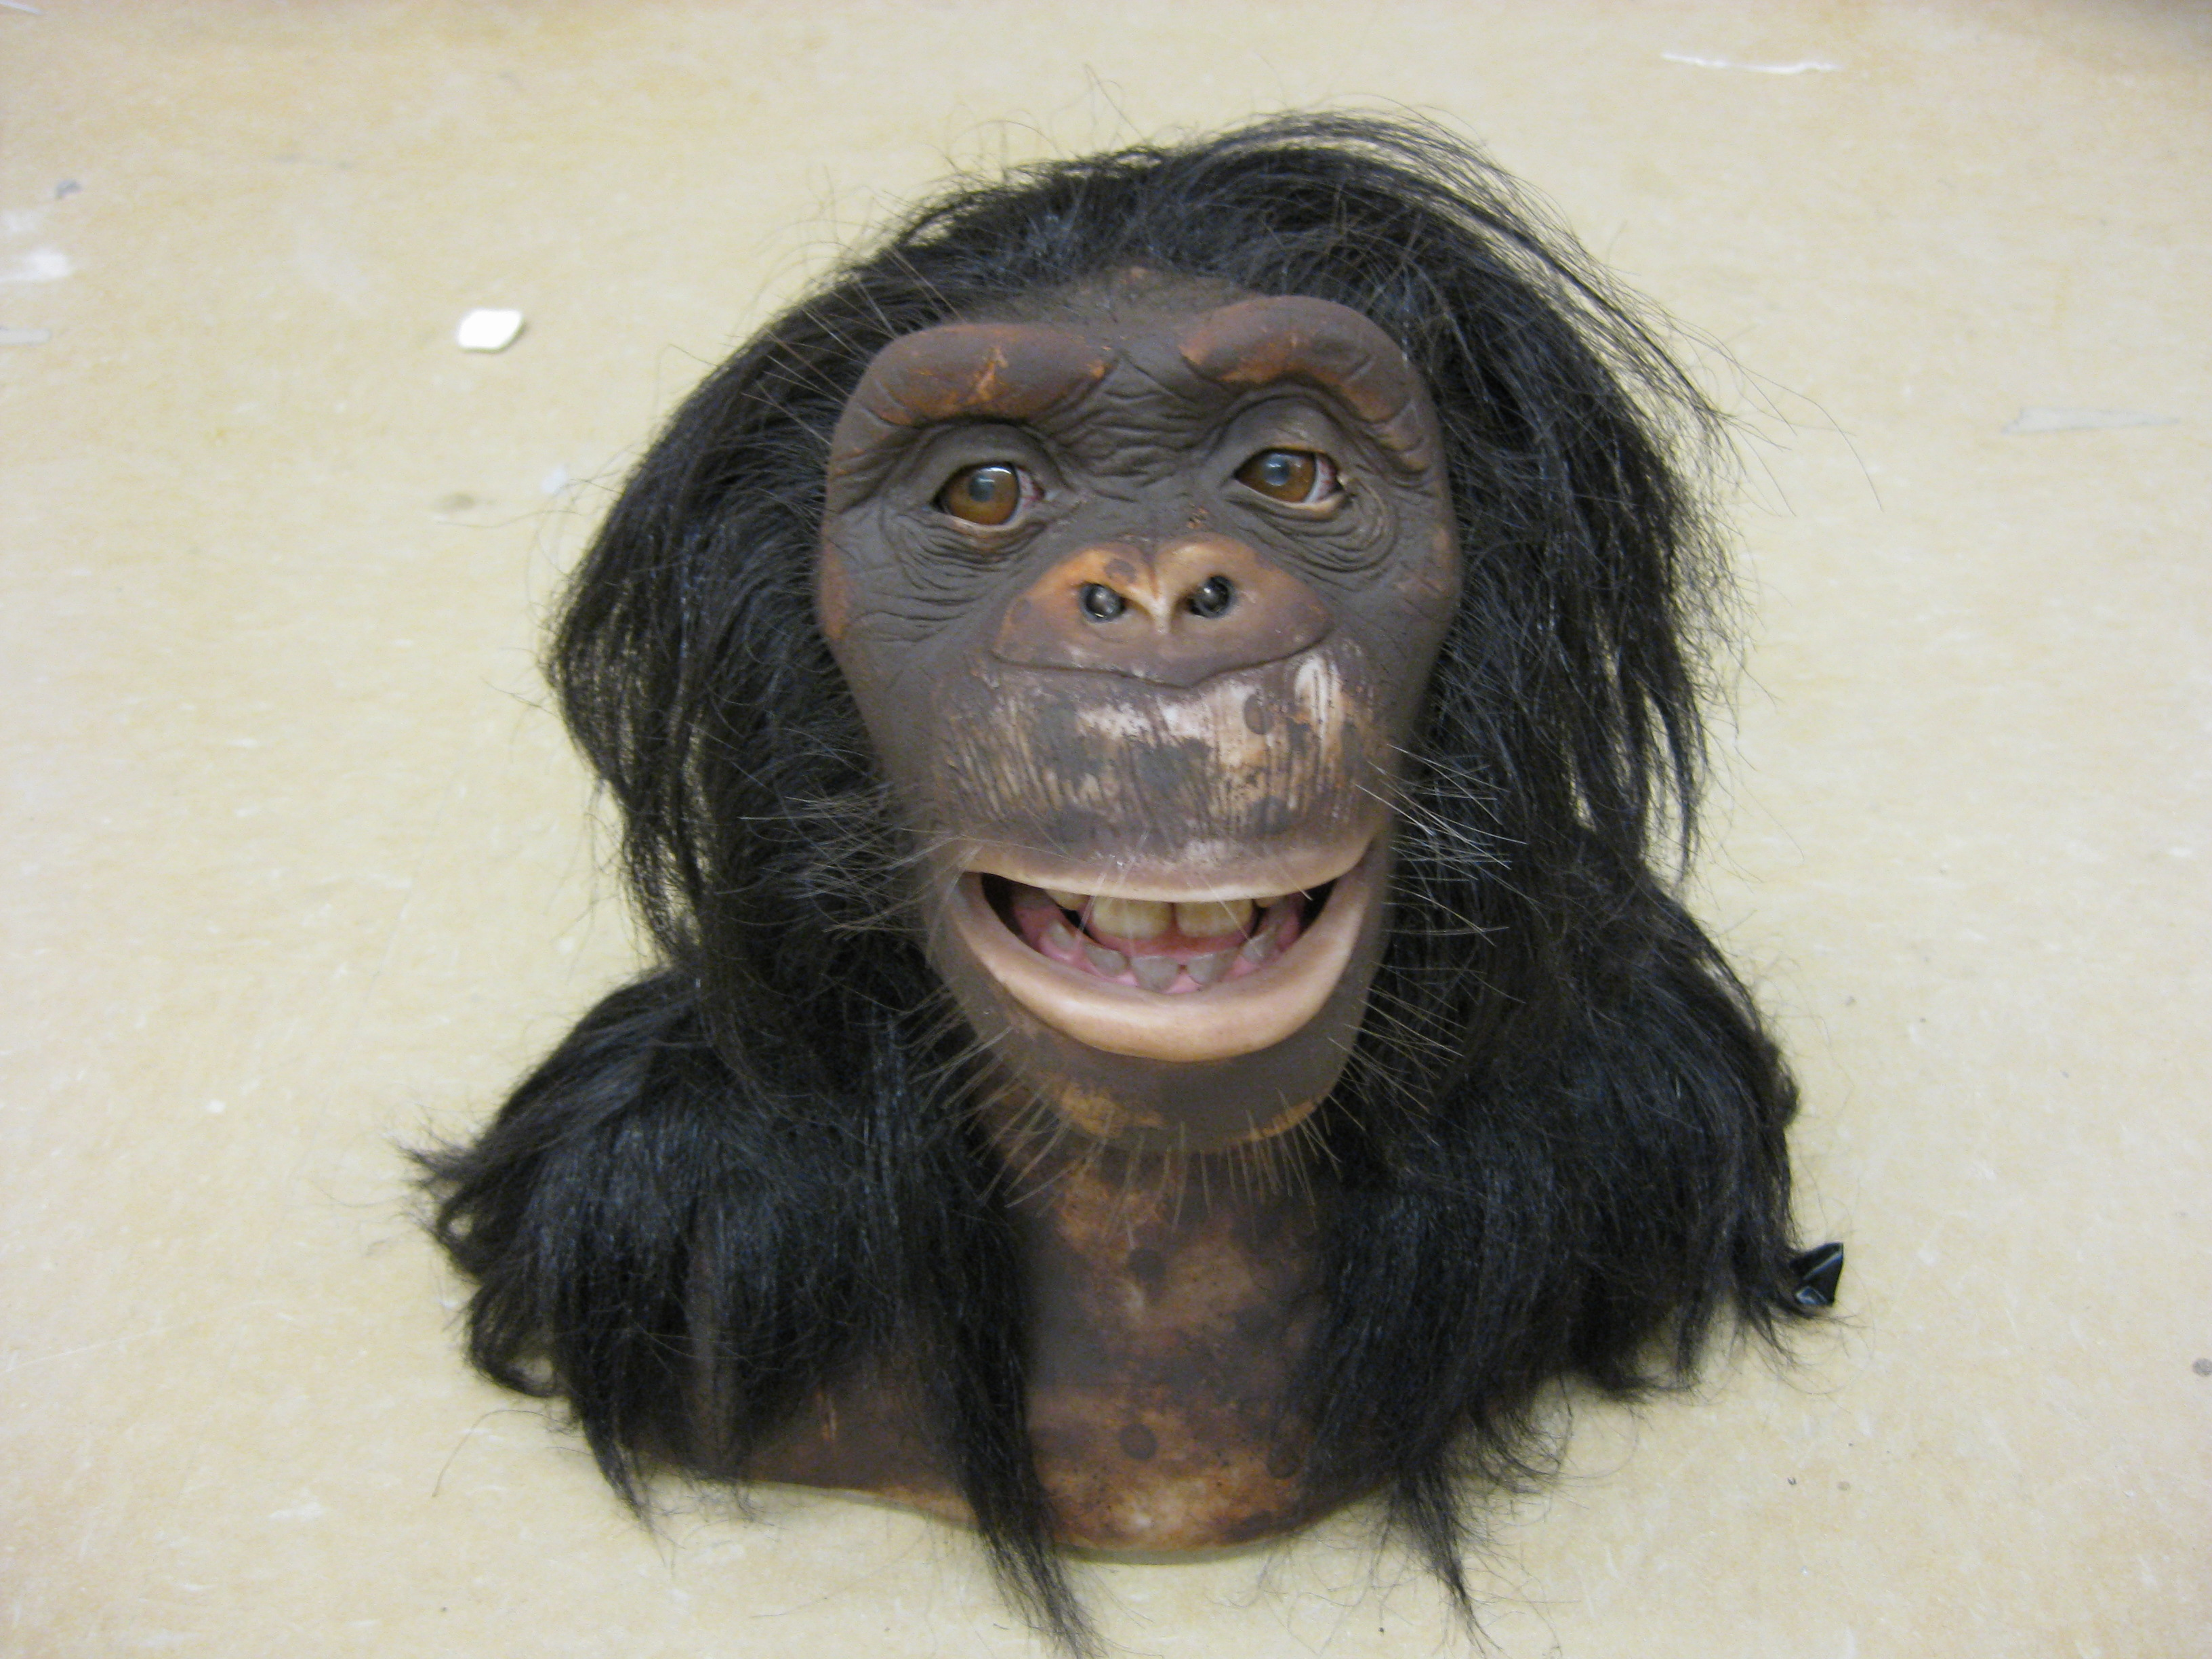
\includegraphics[width=0.8\textwidth]{chimp}
	\caption{The WowWee Alive Chimpanzee (Jiuguang Wang / CC BY-SA).}
	\label{fig:chimp}
\end{figure}

\vfill

\noindent \small{\textit{
The latest version of this document can be found online at \url{https://github.com/jpsheehan/chimp-report/blob/master/report.pdf}.
}}

\newpage

% https://en.wikipedia.org/wiki/WowWee_Alive_Chimpanzee

\section{Introduction}

The Alive Chimpanzee is a toy designed by WowWee Alive, a division of toy-maker WowWee Limited\footnote{\url{https://wowwee.com/}}.
It includes eight motors and nine sensors that allow it to mimic a real chimpanzee.
The original product included an embedded system that would allow the Chimpanzee to be operated by remote control or autonomously via its sensors.

A modified version of the Alive Chimpanzee has been donated to the University of Canterbury.
This modified chimpanzee has had its original control board removed.
Instead, the sensors and motor control lines are wired to a set of pin headers.
The goal of this project is to create an embedded system to allow the Alive Chimpanzee's motors to be controlled via software running on another system via some connection.

\section{Background}

\subsection{Inspection}

The base of the product contains the power switch, battery housings, and power socket.
It was apparent that the product runs on a $\SI{6}{\volt}$ DC power supply, either by four D-size batteries, or a centre-positive $\SI{6}{\volt}$ ($\SI{3.5}{\ampere}$) barrel-jack connector.
The FCC application for the radio transmitter included the user manual\footnote{\url{https://apps.fcc.gov/eas/GetApplicationAttachment.html?id=589802}}.
This provided information about the general operation of the device, including the location and purpose of the internal sensors and motors.

The motors provide a high level of control over the chimpanzee's facial expressions.
Each motor is a standard DC type and includes a feedback signal that is used to determine the angle of the actuated part.
The following functions are provided by the motors:
\begin{itemize}
	\item Head yaw control.
	\item Head pitch control.
	\item Jaw control.
	\item Upper lip control.
	\item Shared eyebrow control.
	\item Shared eyelid control.
	\item Shared eye direction control (requires seperate motors for horizontal and vertical directions).
\end{itemize}

Along with the motor feedback lines, the following sensors are included:
\begin{itemize}
	\item Two infra-red sensors (one in each nostril).
	\item Chin touch sensor.
	\item Front-of-head touch sensor.
	\item Back-of-head touch sensor.
	\item Two microphones (one in each ear).
	\item Two touch sensors (one in each ear).
\end{itemize}

There is also a speaker located in the neck of the product.

\subsection{Hardware Interface}

The modified chimpanzee provides its inputs, outputs, and power lines with a 2-way 25-pin male pin header (figure \ref{fig:pinheader}).
Many of the pins are not connected to any signals and some are still unknown.

\begin{figure}[h]
	\center
	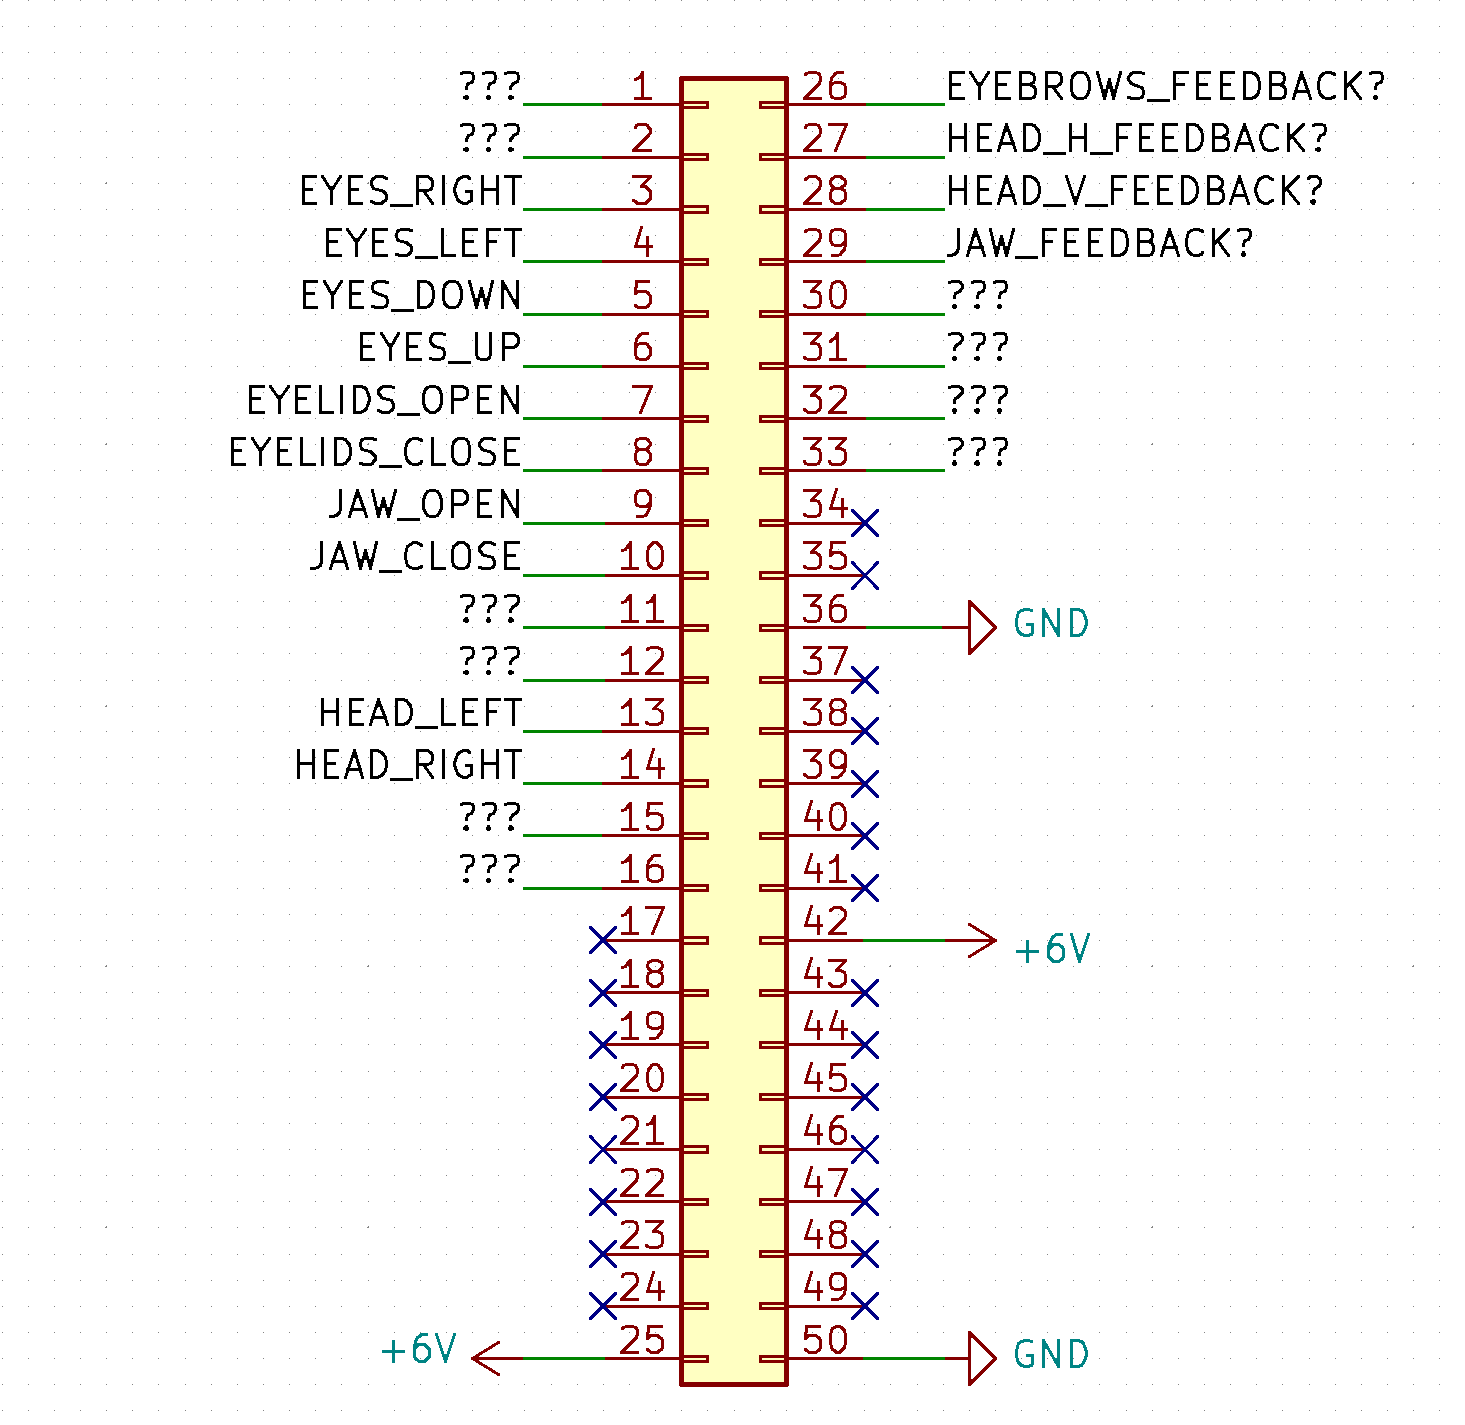
\includegraphics[width=0.6\textwidth]{pinheader}
	\caption{The pin header as viewed from the top.}
	\label{fig:pinheader}
\end{figure}

\section{Method}

A development board was opted to be used instead of a bare microcontroller.
This was done to speed up the time taken to prototype a solution.

The type of microcontroller used in this project is constrained by the number of inputs and outputs (table~\ref{tab:gpio}).
For meeting the primary goal of this project, 8 ADC inputs and 8 digital outputs are required.
To meet these requirements, an Arduino Mega (figure \ref{fig:arduino}) was chosen as the development board.

% include image of Arduino Mega
\begin{figure}[h]
	\center
	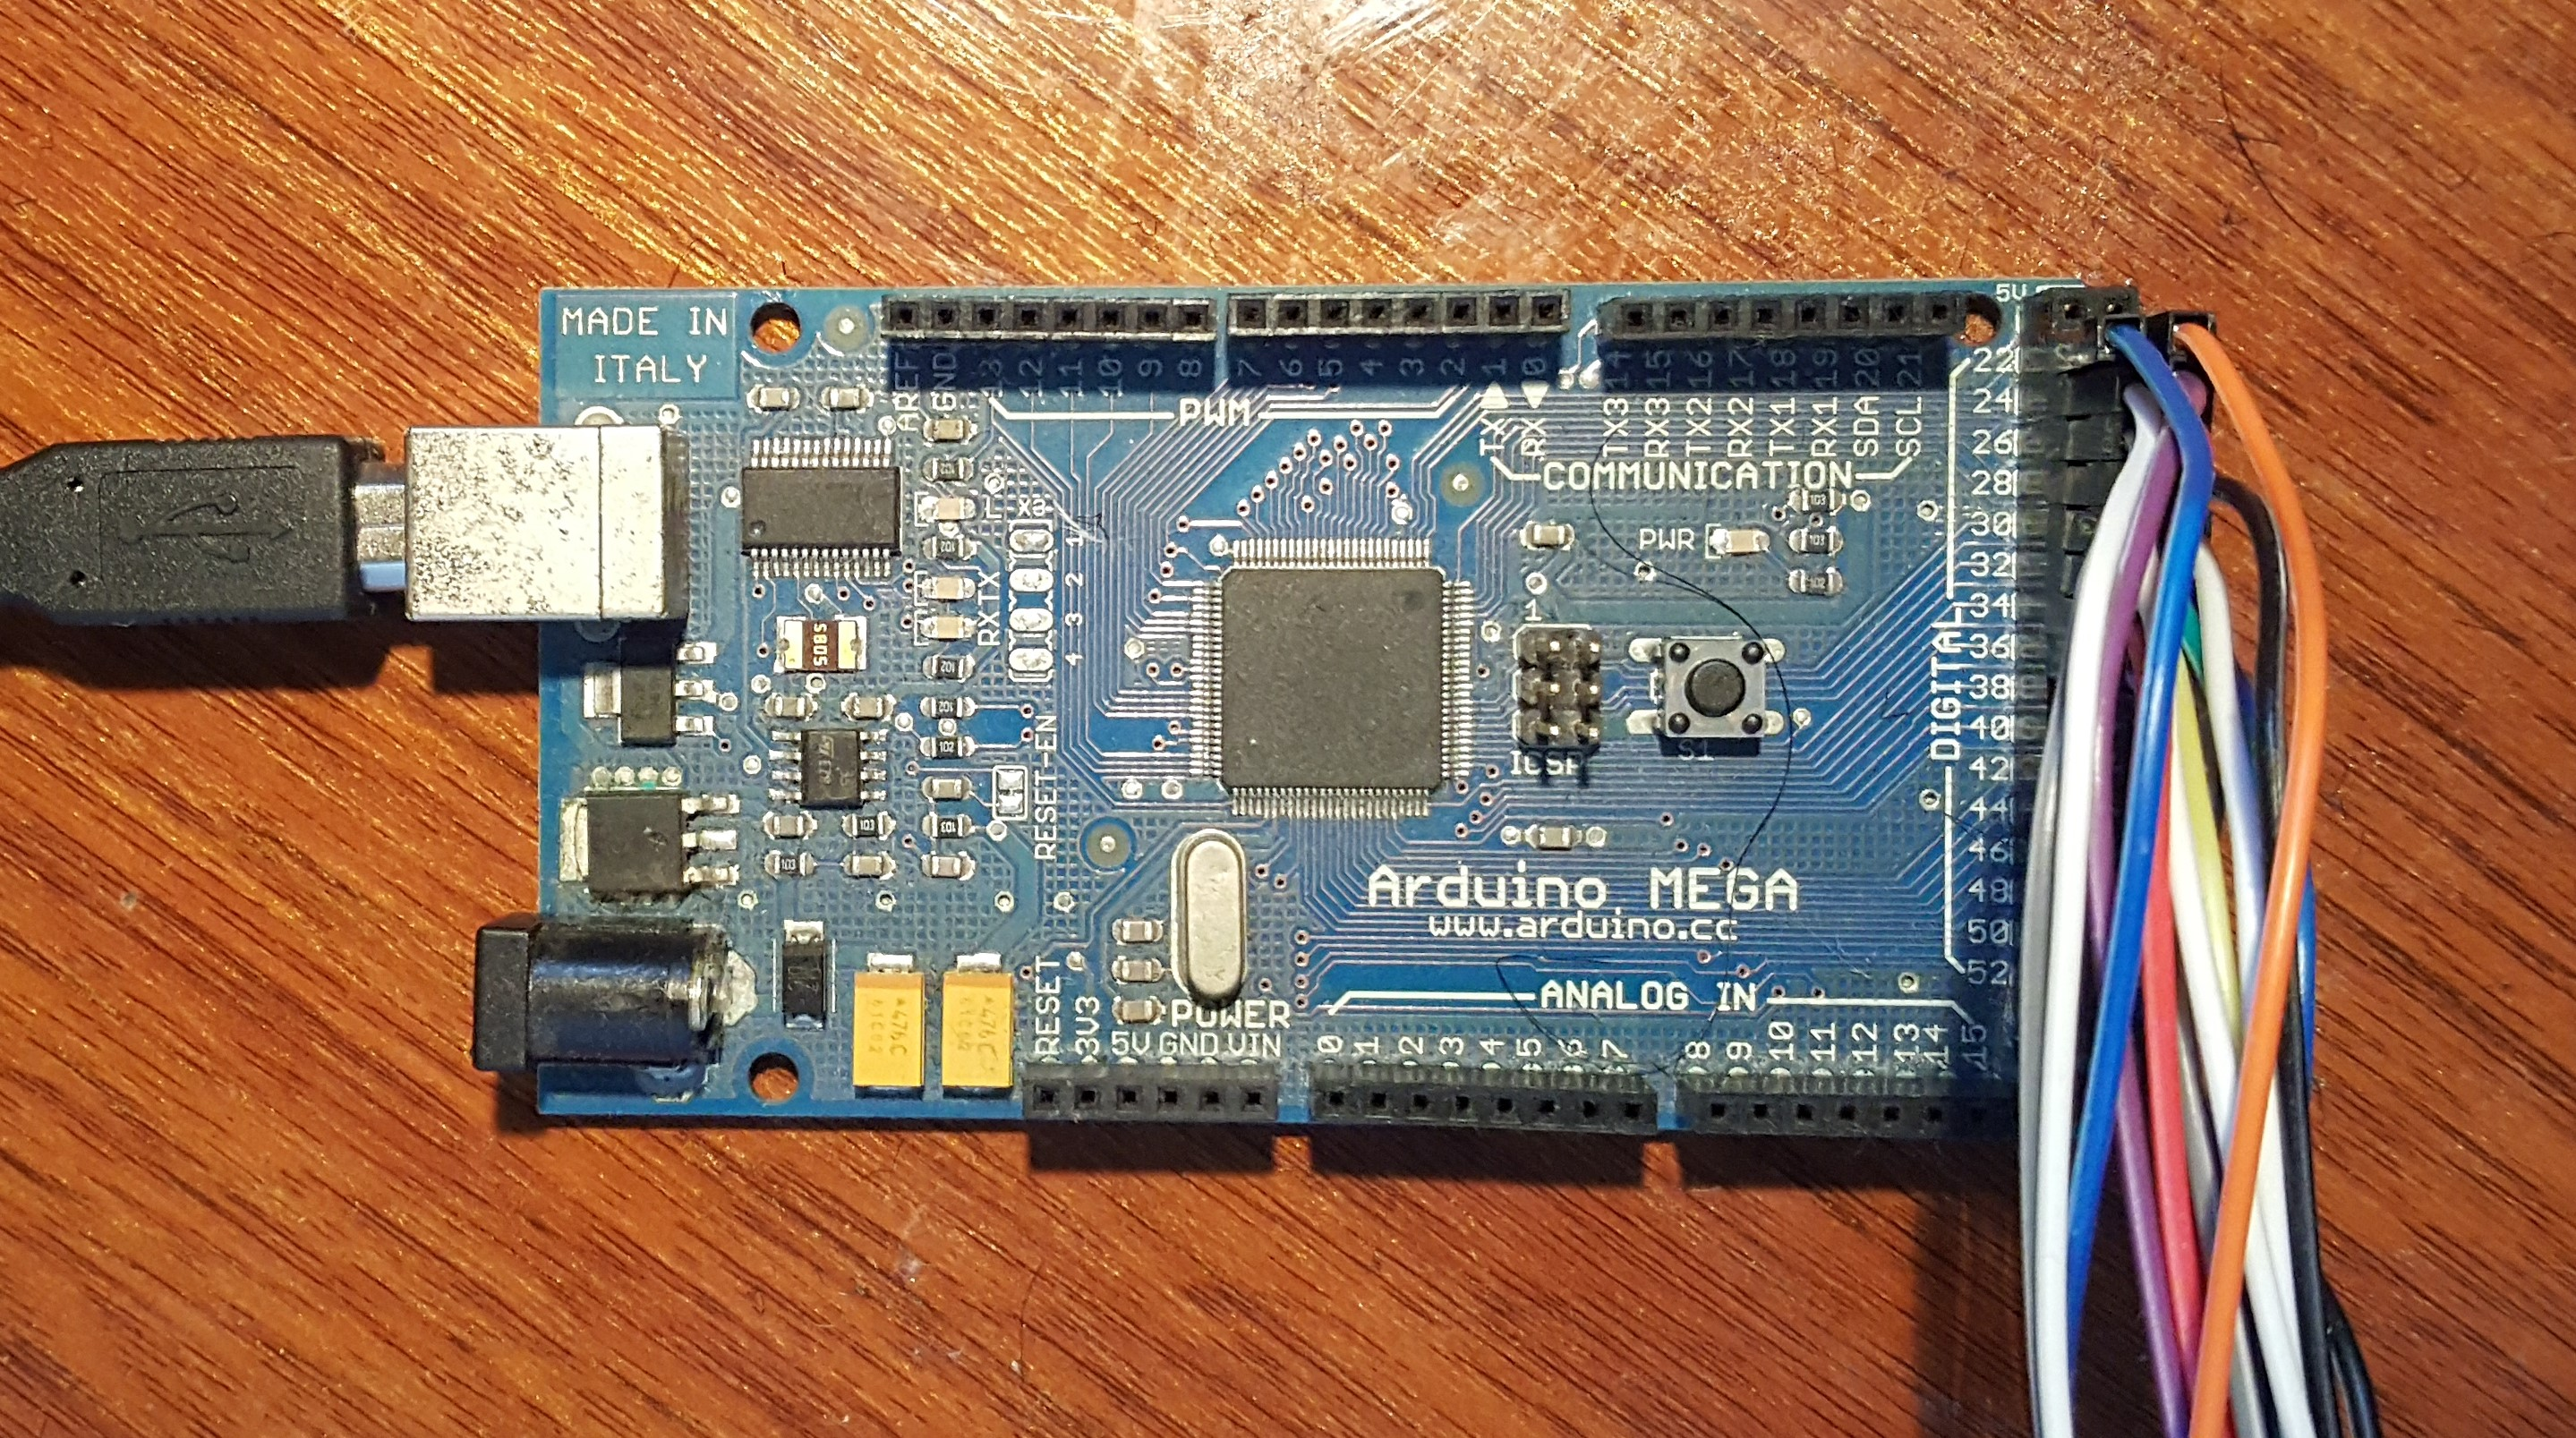
\includegraphics[width=0.6\textwidth]{arduino}
	\caption{The Arduino Mega connected to the motor pins of the chimpanzee.}
	\label{fig:arduino}
\end{figure}

\begin{table}[h]
	\caption{The required inputs and outputs (relative to the microcontroller).}
	\centering
	\begin{tabular}{ |c|c|c| }
		\hline
		\textbf{Signal} & \textbf{Type} & \textbf{Direction} \\
		\hline
		Head yaw motor feedback & Analogue & Input \\
		Head pitch motor feedback & Analogue & Input \\
		Jaw motor feedback & Analogue & Input \\
		Upper lip motor feedback & Analogue & Input \\
		Eyebrow motor feedback & Analogue & Input \\
		Eyelid motor feedback & Analogue & Input \\
		Horizontal eye motor feedback & Analogue & Input \\
		Vertical eye motor feedback & Analogue & Input \\
		Head yaw motor control & Digital & Output \\
		Head pitch motor control & Digital & Output \\
		Jaw motor control & Digital & Output \\
		Upper lip motor control & Digital & Output \\
		Eyebrow motor control & Digital & Output \\
		Eyelid motor control & Digital & Output \\
		Horizontal eye motor control & Digital & Output \\
		Vertical eye motor control & Digital & Output \\
		Ground & --- & --- \\
		\hline
	\end{tabular}
	\label{tab:gpio}
\end{table}

\subsection{Motor Control}

The direction of each motor is controlled by an h-bridge.
Each h-bridge has two inputs, one for each direction.
Care should be taken to not drive both h-bridge inputs at the same time to avoid h-bridge ``shoot-through'', this effectively destroys the MOSFETs, rendering the h-bridge non-operational.

After some investigation, it was discovered that the h-bridges for the head pitch, head yaw, eye pitch, and upper lip were not working.
This may have been the result of h-bridge shoot-through or some other defect.
This will need to be investigated further and fixed.

The digital inputs can also be controlled via a PWM signal.
This allows the motors to operate at a slower speed.
For this project PWM was not used.
However, this could be useful for a future revision of the firmware.

\subsection{Motor Feedback}

For this proof-of-concept the motor feedback lines were not used as they could not reliably detect the position of their respective motors.

\subsection{Firmware}

A simple firmware package was designed using the Arduino IDE to provide basic motor control for the product.
It is written in C and C++ and provides a serial interface to a PC or other device. 
It does not attempt to operate the h-bridges that are faulty (however this can be enabled easily).

Table \ref{tab:pinmap} shows the expected connections between the Arduino Mega and the chimpanzee pin header for the firmware to work.

\begin{table}[h]
	\caption{The expected pin mapping between the Arduino and the chimpanzee.}
	\centering
	\begin{tabular}{ |c|c|c| }
		\hline
		\textbf{Signal} & \textbf{Arduino Pin} & \textbf{Chimp Pin} \\
		\hline
		??? & 22 & 1 \\
		??? & 23 & 2 \\
		Eyes Right & 24 & 3 \\
		Eyes Left & 25 & 4 \\
		Eyes Down & 26 & 5 \\
		Eyes Up & 27 & 6\\
		Eyelids Open & 28 & 7 \\
		Eyelids Close & 29 & 8 \\
		Jaw Open & 30 & 9 \\
		Jaw Close & 31 & 10 \\
		Eyebrows Down & 32 & 11 \\
		Eyebrows Up & 33 & 12 \\
		Head Left & 34 & 13 \\
		Head Right & 35 & 14\\
		??? & 36 & 15 \\
		??? & 37 & 16 \\
		Ground & GND & 36 \\
		\hline
	\end{tabular}
	\label{tab:pinmap}
\end{table}


\subsection{Software}

A simple API for interacting with the firmware via a serial connection on a host PC is provided.
It is written in Python (version 3) but can be implemented relatively easily in another language.

An example program with a GUI (figure \ref{fig:gui}) is included to demonstrate how to call the API functions.

The firmware and software can be found in the chimp-code GitHub repository\footnote{\url{https://github.com/jpsheehan/chimp-code/}}.

\begin{figure}[H]
	\center
	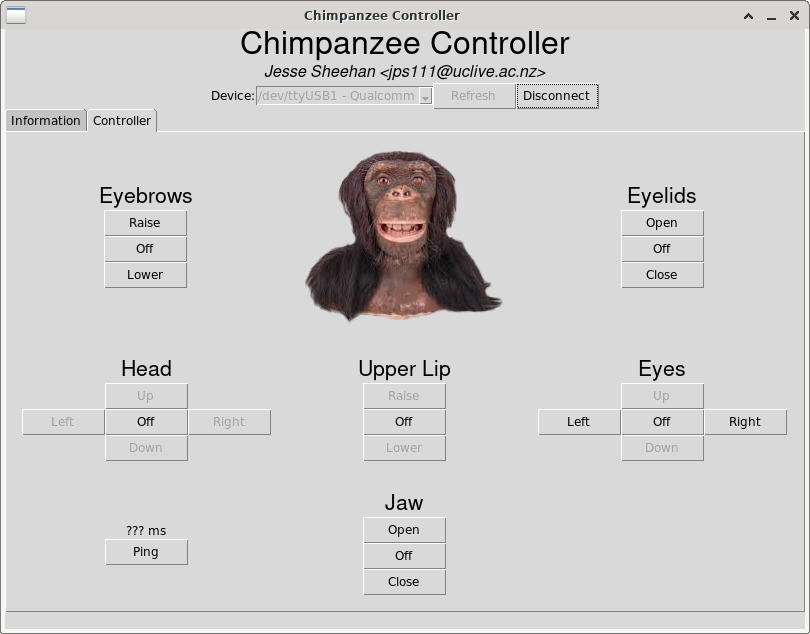
\includegraphics[width=0.7\textwidth]{gui}
	\caption{The demonstration graphical user interface.}
	\label{fig:gui}
\end{figure}

\section{Results}

The chimpanzee was powered by a $\SI{6}{\volt}$ bench power supply and connected to a laptop via a USB cable (figure \ref{fig:test}).
The laptop was running a Linux-based operating system and Python version 3.8.

The demonstration program allows the user to control the chimpanzee via a GUI using a mouse. Some functionality is disabled due to the malfunctioning h-bridges.

\begin{figure}[H]
	\center
	\includegraphics[width=0.6\textwidth]{test}
	\caption{The testing setup with chimpanzee and power supply.}
	\label{fig:test}
\end{figure}

\section{Conclusion}

A microcontroller was used to allow a toy chimpanzee head to be controlled via a computer.
It was found that some of the motor drive circuitry was non-functional and thus could not be activated.
Firmware was written in C/C++ to control the remaining motors, this functionality is exposed via a serial protocol.
A software API was written in Python to interact with the microcontroller via the serial protocol.
A demonstration program was included to show how to interact with the API.

The project is functional enough to be included and used in other projects such as computer vision, etc.

\subsection{Future Research}

The following tasks should be undertaken to improve the results of the project:
\begin{itemize}
	\item A discrete $\SI{6}{\volt}$ power supply should be purchased so that a bench supply is not needed.
	\item The 4 broken h-bridges should be fixed.
	\item The motor feedback signals should be used to provide finer control of the motors.
	\item The motors could be controlled via PWM to allow for motor speed control.
	\item All of this functionality should be exposed via the firmware via the serial protocol and software API.
\end{itemize}

\end{document}
